\section{System Architecture}

A system architecture diagram is created to help to understand the system as well as its components better. 

\begin{figure}[h]
 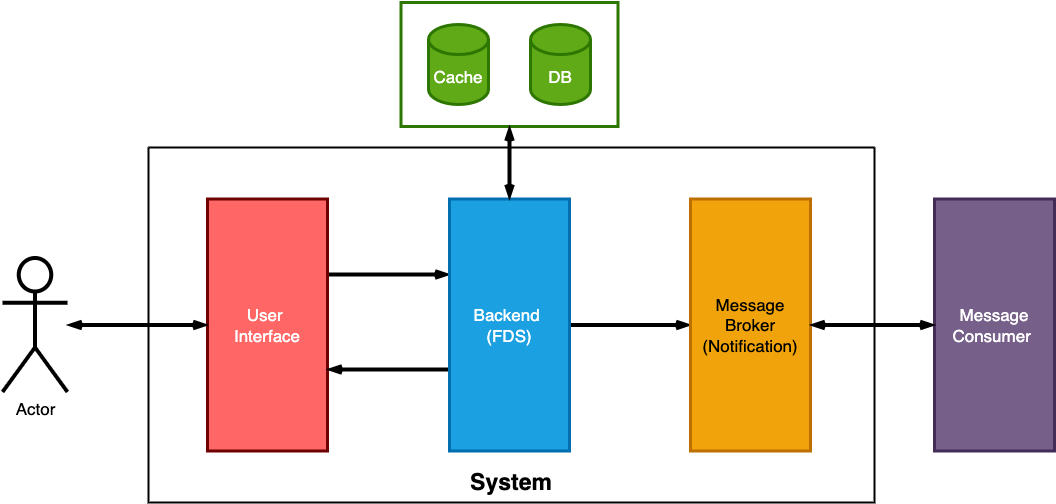
\includegraphics[width=\textwidth]{diagrams/system.png}
 \caption{System architecture diagram}
\end{figure}
 
The system diagram visualizes the components of the system and their interaction with each other. Internally, the system contains 3 independent components; user interface (UI), fraud detection service (FDS) and a message broker (notification system). 
Externally, the system would interact with a database and optionally a cache memory\footnote{Cache memories are small, but extremely fast memory used in computer systems to store information that are going to be accessed in a small timeframe \autocite{smith-1982}.}  to persist information needed for the validation process. The diagram also visualizes an external system (\emph{message consumer}) which is indeed out of the system's scope, but plays an important role to determine which action should be taken on certain events. Further information on the function as well as connection between each component will be discussed on the next section.